% Options for packages loaded elsewhere
\PassOptionsToPackage{unicode}{hyperref}
\PassOptionsToPackage{hyphens}{url}
%
\documentclass[
]{article}
\usepackage{amsmath,amssymb}
\usepackage{iftex}
\ifPDFTeX
  \usepackage[T1]{fontenc}
  \usepackage[utf8]{inputenc}
  \usepackage{textcomp} % provide euro and other symbols
\else % if luatex or xetex
  \usepackage{unicode-math} % this also loads fontspec
  \defaultfontfeatures{Scale=MatchLowercase}
  \defaultfontfeatures[\rmfamily]{Ligatures=TeX,Scale=1}
\fi
\usepackage{lmodern}
\ifPDFTeX\else
  % xetex/luatex font selection
\fi
% Use upquote if available, for straight quotes in verbatim environments
\IfFileExists{upquote.sty}{\usepackage{upquote}}{}
\IfFileExists{microtype.sty}{% use microtype if available
  \usepackage[]{microtype}
  \UseMicrotypeSet[protrusion]{basicmath} % disable protrusion for tt fonts
}{}
\makeatletter
\@ifundefined{KOMAClassName}{% if non-KOMA class
  \IfFileExists{parskip.sty}{%
    \usepackage{parskip}
  }{% else
    \setlength{\parindent}{0pt}
    \setlength{\parskip}{6pt plus 2pt minus 1pt}}
}{% if KOMA class
  \KOMAoptions{parskip=half}}
\makeatother
\usepackage{xcolor}
\usepackage[margin=1in]{geometry}
\usepackage{graphicx}
\makeatletter
\def\maxwidth{\ifdim\Gin@nat@width>\linewidth\linewidth\else\Gin@nat@width\fi}
\def\maxheight{\ifdim\Gin@nat@height>\textheight\textheight\else\Gin@nat@height\fi}
\makeatother
% Scale images if necessary, so that they will not overflow the page
% margins by default, and it is still possible to overwrite the defaults
% using explicit options in \includegraphics[width, height, ...]{}
\setkeys{Gin}{width=\maxwidth,height=\maxheight,keepaspectratio}
% Set default figure placement to htbp
\makeatletter
\def\fps@figure{htbp}
\makeatother
\setlength{\emergencystretch}{3em} % prevent overfull lines
\providecommand{\tightlist}{%
  \setlength{\itemsep}{0pt}\setlength{\parskip}{0pt}}
\setcounter{secnumdepth}{-\maxdimen} % remove section numbering
\usepackage{multicol}
\usepackage{longtable}
\setlength{\columnsep}{1cm}
\usepackage{booktabs}
\usepackage{array}
\usepackage{float}
\usepackage{longtable}
\ifLuaTeX
  \usepackage{selnolig}  % disable illegal ligatures
\fi
\usepackage{bookmark}
\IfFileExists{xurl.sty}{\usepackage{xurl}}{} % add URL line breaks if available
\urlstyle{same}
\hypersetup{
  pdftitle={Análisis de Variables que Influyen en la Inversión, Innovación e Implementación de la Inteligencia Artificial},
  pdfauthor={Adrada Isabel, De la Peña Juan, Terán Federico, Troncoso Samuel},
  hidelinks,
  pdfcreator={LaTeX via pandoc}}

\title{Análisis de Variables que Influyen en la Inversión, Innovación e
Implementación de la Inteligencia Artificial}
\author{Adrada Isabel, De la Peña Juan, Terán Federico, Troncoso Samuel}
\date{}

\begin{document}
\maketitle

\begin{multicols}{2}

\section{Resumen}
...
...

\section{Key words}
...
...

\section{Introducción}
Las compañıas involucradas en el desarrollo tecnológico con inteligencia artificial (IA) necesitan identificar los países y regiones con mayor potencial de adopción e implementacio ́n de estas herramientas. Este análisis es crucial para la toma de decisiones estratégicas, la definición de mercados objetivo y la planificación de la expansión geográfica. El objetivo general de este estudio radica en identificar las variables con un mayor grado de influencia en el nivel de inversión, innovación e implementación de la inteligencia artificial, reflejado en el AI global index de diferentes regiones del mundo, por lo cuál se buscará determinar la influencia de los factores relacionados con la inversión mediante el índice Commerce, la influencia de los factores relacionados a la innovación mediante el índice Research, la influencia de los factores relacionados a la implementación mediante el índice Talent y la influencia de los factores relacionados con la ubicación geográfica del país mediante la categorización por Región.




\section{Métodos}
Para la definición de las variables a estudiar a partir de la base de datos AI Global Index trabajada en el presente estudio, se relalizó una exploración preliminar de los datos en la Tabla 1, donde se nombran las variables, se clasifican como cualitativas o cuantitativas, se categorizan como continuas o discretas, o nominal u ordinal según el caso y se realiza una descripción de las mismas.

\end{multicols}

\renewcommand{\arraystretch}{1.5}
\begin{footnotesize}
\begin{longtable}[t]{lllp{8cm}}
\caption{\label{tab:tabla1}Variables y su clasificación}\\
\toprule
Variable & Clasificación & Categorización & Descripción\\
\midrule
Country & Cualitativa & Nominal & Nombre del país donde se evalúa el AI Global Index.\\
Talent & Cuantitativa & Continua & Indicador de disponibilidad de profesionales calificados para la provisión de soluciones de inteligencia artificial.\\
Infraestructure & Cuantitativa & Continua & Indicador de fiabilidad y la escala de la infraestructura de acceso, desde la electricidad e Internet, hasta las capacidades de superintarmética.\\
Operating Enviroment & Cuantitativa & Continua & Indicador del contexto regulatorio y la opinión pública en torno a la inteligencia artificial.\\
Research & Cuantitativa & Continua & Indicador del alcance de la investigación especializada y los investigadores; investigando la cantidad de publicaciones y citas en revistas académicas creíbles.\\
\addlinespace
Development & Cuantitativa & Continua & Indicador de desarrollo de plataformas y algoritmos fundamentales en los que se basan los proyectos innovadores de inteligencia artificial.\\
Government Strategy & Cuantitativa & Continua & Indicador de la profundidad del compromiso del gobierno nacional con la inteligencia artificial; investigando los compromisos de gasto y las estrategias nacionales.\\
Commercial & Cuantitativa & Continua & Indicador del nivel de actividad de puesta en marcha, inversión e iniciativas comerciales basadas en la inteligencia artificial.\\
Total Score & Cuantitativa & Continua & Indicador AI Global Index que compara a las naciones en su nivel de inversión, innovación e implementación de la inteligencia artificial.\\
Region & Cualitativa & Nominal & Agrupacion de países según su localización geográfica en regiones.\\
\addlinespace
Cluster & Cualitativa & Nominal & Agrupación de países según su historia de incursión en el desarrollo de tecnología relacionada con la Inteligencia Artificial.\\
Income Group & Cualitativa & Ordinal & Nivel de ingresos presentado en el país.\\
Political Regime & Cualitativa & Nominal & Tipo de régimen político presentado en el país.\\
\bottomrule
\end{longtable}

\end{footnotesize}\renewcommand{\arraystretch}{1}

\begin{multicols}{2}


Posteriormente, con el propósito de indentificar las posibles variables con un mayor grado de influencia en el nivel de inversión, innovación e implementación de la inteligencia artificial, se elaboró la figura 1, la cuál presenta una comparación de las distribuciones de las variables y sus respectivos coeficientes de correlación lineal de Pearson con el fin de reconocer los índices que presentan un mayor valor respecto al AI Global Index (Total Score), los cuáles fueron Commerce para el nivel de inversión, Research para la innovación y Talent para la implemetación. 




\begin{center}
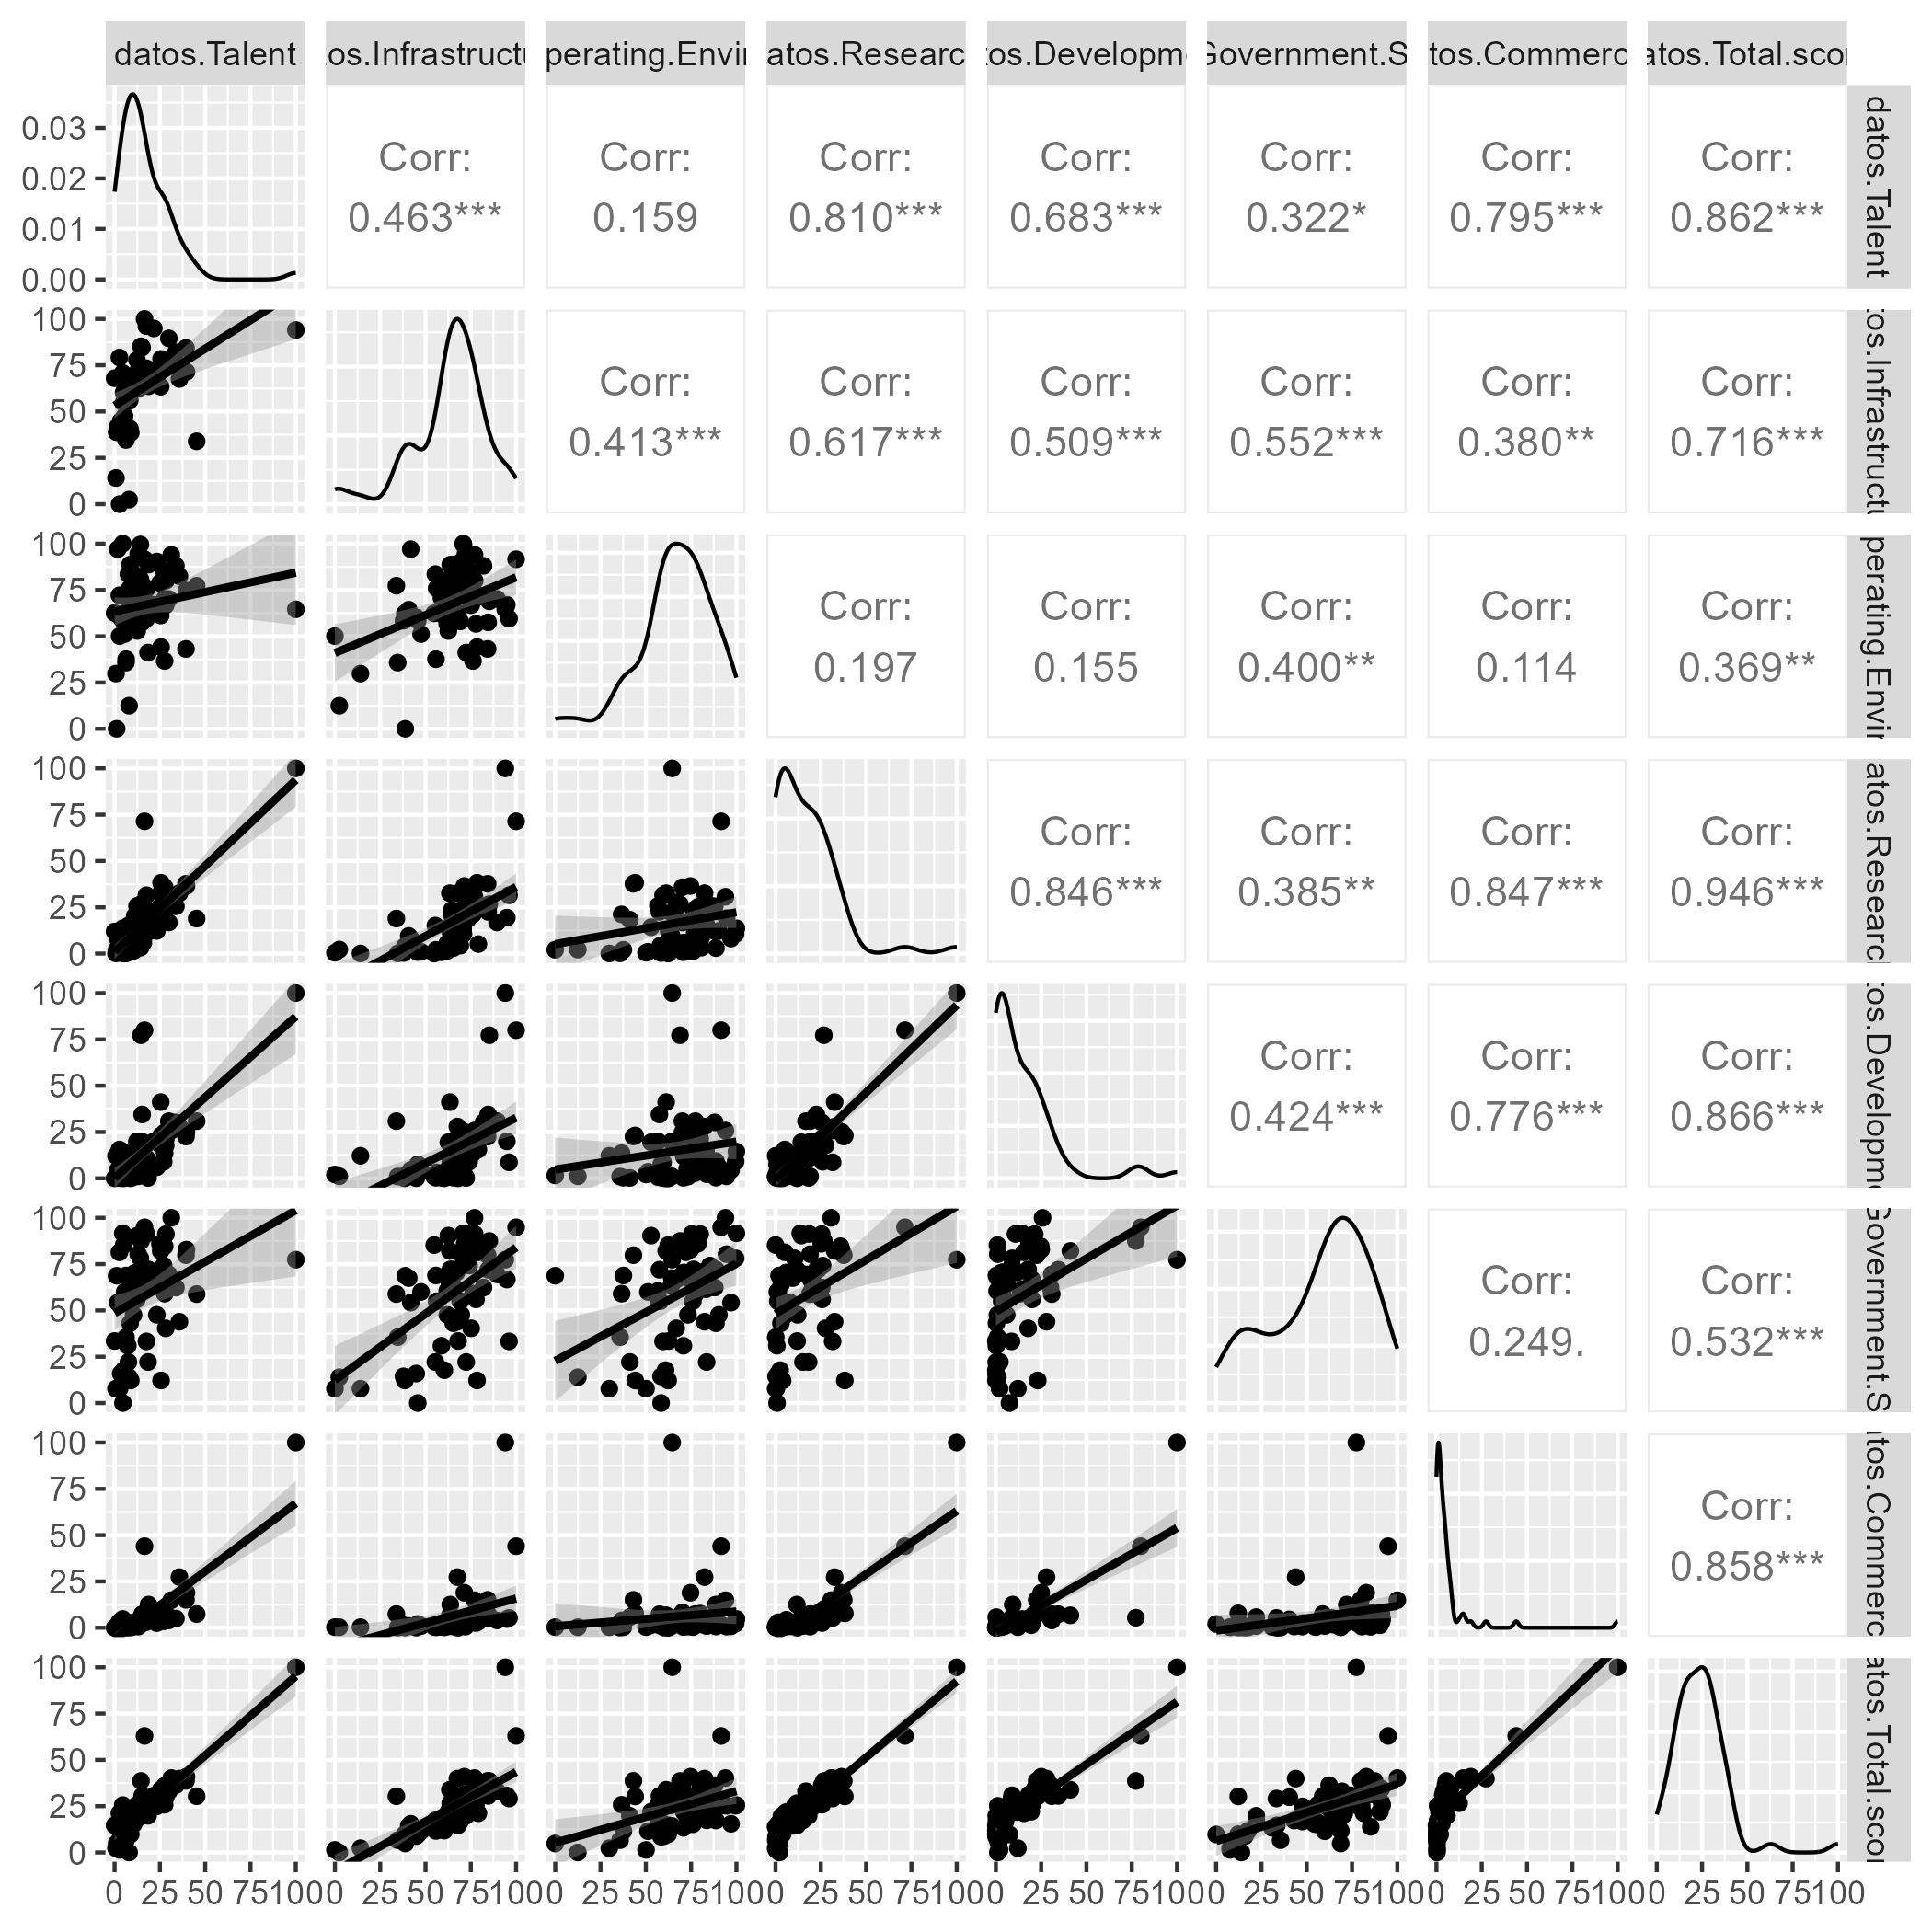
\includegraphics[width=\linewidth]{figura1.png}
\end{center}
Figura 1. Correlación lineal de Pearson índices.

Posteriormente, se realizó ... 
... para cada uno de los índices con el fin de ...

\section{Resultados}
En la Tabla 2 se presentan las medidas de tendencia central, posición, disperción, covarianza y correlación lineal de Pearson con respecto al Total Score (AI Global Index) de las variables cuantitativas Índice Commerce, Research y Talent. 

Todos los índices tienen un mínimo de 0 y un máximo de 100, por lo tanto, todos los rangos son también de 100, lo cuál no brinda mucha información acerca de la distribución de los datos, sin embargo facilita la comparación entre las estadísticas de las diferentes variables. El índice Commerce tiene la media más baja con 6.172, Talent y Research una media similiar al rededor de 16 y Total Score la mayor media con 23.915, sin embargo en todos los casos los datos son altamente heterogéneos, considerando que el coeficiente de variación de todas las variables es mayor al 50%, e incluso, para el caso de Commerce este supera el 100%. Para los índices con menos de tres modas se identifica que estas están alejadas de la media, y lo mismo sucede con la mediana, lo cuál es un indicador de que los índices no se distribuyen de normalmente. 

En el caso de la covarianza, esta es positiva para todas las variables, lo cuál plantea la posibilidad de que estas tengan una relación lineal directa con el índice Total Score. Esto es confirmado con el coeficiente de correlación de Pearson, donde un valor superior a 0.8 indica hay una relación muy significativa, lo cuál es cierto para todos los casos, donde la variable Research presenta el indicador más alto con un coeficiente de 0.946.

\end{multicols}

\renewcommand{\arraystretch}{1.5}
\begin{footnotesize}
\begin{longtable}[t]{lllll}
\caption{\label{tab:resultados}Estadísticas descriptivas por variable}\\
\toprule
Estadísticas & Índice\_Commerce & Índice\_Talent & Índice\_Research & Índice\_Total\_Score\\
\midrule
Media & 6.172 & 16.803 & 16.61 & 23.915\\
Moda & 0.31 & > 3 modas & 32.63 & > 3 modas\\
Desviación estándar & 14.03 & 15.215 & 17.414 & 15.124\\
Mínimo & 0 & 0 & 0 & 0\\
Q1 & 0.698 & 7.365 & 3.033 & 14.805\\
\addlinespace
Mediana & 2.585 & 13.445 & 12.93 & 23.22\\
Q3 & 5.308 & 24.567 & 25.413 & 30.488\\
Máximo & 100 & 100 & 100 & 100\\
Rango & 100 & 100 & 100 & 100\\
IQR & 4.61 & 17.202 & 22.38 & 15.683\\
\addlinespace
CV & 227.317 & 90.549 & 104.84 & 63.241\\
Covarianza - Total Score & 182.046 & 198.343 & 249.108 & NA\\
Correlación lineal - Total Score & 0.858 & 0.862 & 0.946 & NA\\
\bottomrule
\end{longtable}

\end{footnotesize}\renewcommand{\arraystretch}{1}

\begin{multicols}{2}

Para otener una perspectiva más amplia de la distribución de los datos, en la Tabla 3 se presentan las frecuencias univariadas de las variables cuantitativas Índice Commerce, Research y Talent. 

...

\subsection{Índice Commerce}
tabla de frecuencia bivariada (indice vs total socore)
tabla con covarianza y coeficiente de correlacion de pearson
histograma
ojiva
diagrama de cajas y bigotes

\subsection{Índice Research}
tabla de frecuencia bivariada (indice vs total socore)
histograma
ojiva
diagrama de cajas y bigotes

\subsection{Índice Talent}
tabla de frecuencia bivariada (indice vs total socore)
histograma
ojiva
diagrama de cajas y bigotes

\subsection{Región}
tabla de frecuencia univariada
tabla de frecuencia bivariada (region y total score)
diagrama de torta

\section{Análisis de resultados}

\section{Conclusiones}
\section{Referencias}

\end{multicols}

\end{document}
